\selectlanguage{italian}%

\section{Simulazione}

\begin{figure}[H]
	\centering
	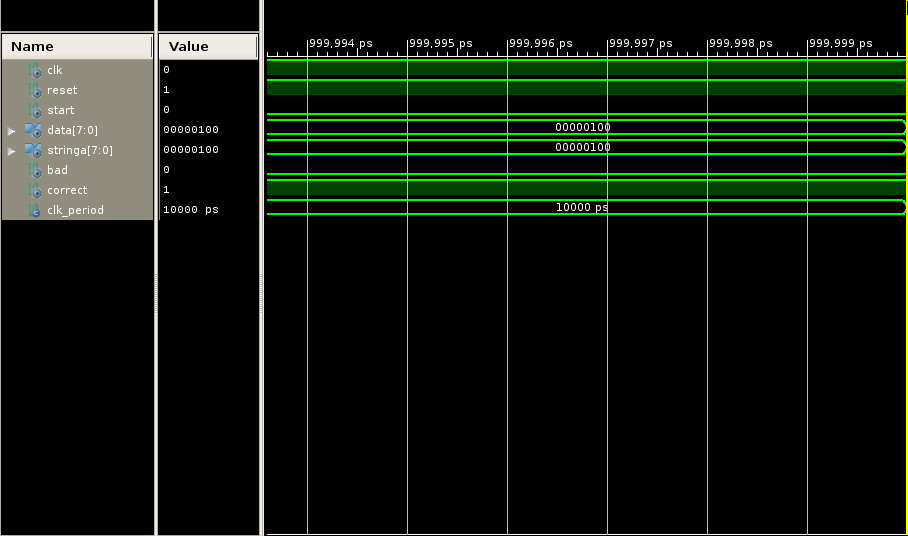
\includegraphics[scale=0.5]{esercizio07/images/correct.png}
	\caption{Stringa riconosciuta correttamente}
\end{figure}

\begin{figure}[H]
	\centering
	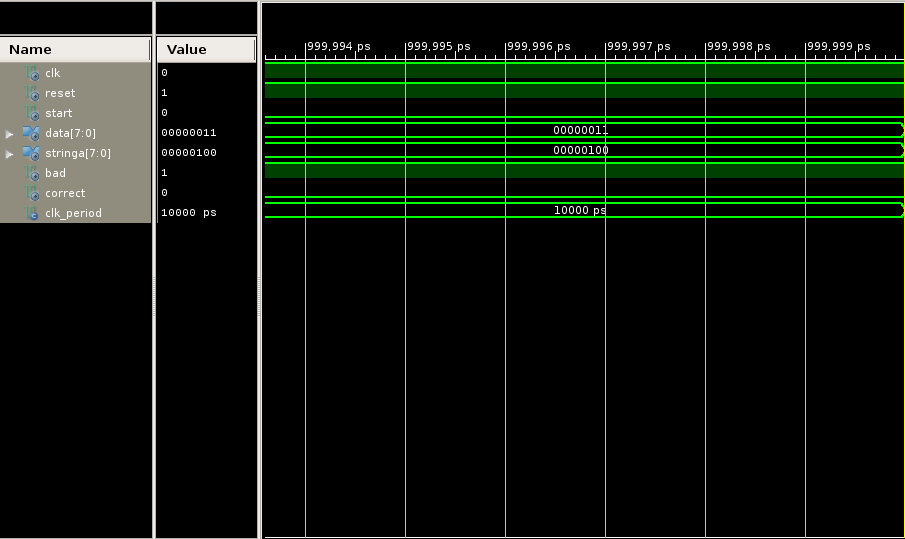
\includegraphics[scale=0.5]{esercizio07/images/bad.png}
	\caption{Stringa non riconosciuta}
\end{figure}

Nei due esempi: in alto, viene mostrato un caso in cui la stringa
da riconoscere � quella in ingresso sono le stesse in basso invece,
in cui le due stringhe sono dissimili.\selectlanguage{italian}%

